\documentclass[final, 12pt, oneside, openright]{class_diss}
\usepackage[utf8]{inputenc}
\usepackage[T1]{fontenc}
\usepackage[spanish, es-tabla]{babel}
\selectlanguage{spanish}
\usepackage{eurosym}
\usepackage{listings}
\usepackage{cancel}
\usepackage{algorithm}
\usepackage{algorithmic}
\usepackage{      amsmath}
\usepackage{     graphicx}
\usepackage{amsxtra}
\usepackage{amssymb}
\usepackage{amsthm}
\usepackage{latexsym}
\usepackage{enumerate}
\usepackage{float}
\usepackage{rotating}
\usepackage[usenames]{color}
\usepackage[table]{xcolor}
\definecolor{  Pink}{rgb}{1.0, 0.5, 0.5}
\definecolor{Maroon}{rgb}{0.8, 0.0, 0.0}
\usepackage[sort&compress]{natbib}
\usepackage[pdftex, plainpages=false, pdfpagelabels]{hyperref}
\usepackage{url}

\hypersetup{
    linktocpage=true,
    colorlinks=true,
    bookmarks=true,
    citecolor=blue,
    urlcolor=blue,https://www.overleaf.com/project/5db83b575ef1b30001f7a93f
    linkcolor=Maroon,
    citebordercolor={1 0 0},
    urlbordercolor={1 0 0},
    linkbordercolor={.7 .8 .8},
    breaklinks=true,
    pdfpagelabels=true,
}

\topmargin      = -0.56in
\textheight     = 8.60in
\textwidth      = 6.46in
\oddsidemargin  = 0.02in

\begin{document}
    \setcounter{page}{-1}
    \newpage


\thispagestyle{empty}


\begin{center}

    \vspace{1cm}


    {\Large Implementación paralela del Automatic Target Detection and Classification Algorithm haciendo uso de la ortogonalización de Gram Schmidt
    para el análisis de imágenes hiperespectrales}\\

    \vspace{1.5cm}

    {\large Andrés Ortiz Loaiza}\\

    \vspace{1.5cm}

    GRADO EN INGENIERÍA DE COMPUTADORES. FACULTAD DE INFORMÁTICA\\
    UNIVERSIDAD COMPLUTENSE DE MADRID \\


    \vspace{0.65cm}
    \rule{2in}{0.5pt}\\
    \vspace{0.85cm}

    
\includegraphics[height=2.5in]{images/ucm/shield2.jpg}

    \vspace{0.5cm}
    Trabajo Fin de Grado en Ingeniería de Computadores

    \vspace{0.5cm}

    Madrid, mayo de 2019\\
    \vspace{3cm}

\end{center}

{\raggedleft
    Directores:\\
    \vspace{ 0.5cm}
    González Calvo, Carlos\\
    Bernabé García, Sergio\\
}
    \pdfbookmark[0]{Cover}{PDFCoverPage}
    %\newpage\leavevmode\thispagestyle{empty}\newpage
    \newpage
\thispagestyle{empty}
\begin{center}
{\bf \Huge Agradecimientos}
\end{center}
\vspace{1cm}
\setlength{\baselineskip}{0.8cm}

Gracias a mis profesores por apoyar mis ideas y hacer de este proyecto algo con lo que he podido disfrutar en todo momento.

Por supuesto gracias a mi madre, la persona que siempre ha estado conmigo en todos los momentos buenos y malos de mi vida.
\textit{}
    %\phantomsection
   % \newpage\leavevmode\thispagestyle{empty}\newpage
    %\newpage
    \pagenumbering{roman}
    \setcounter{page}{1}
    \cleardoublepage
    \phantomsection
    \addcontentsline{toc}{chapter}{Índice general}
    \tableofcontents
    \listoffigures
    \listoftables
    \vspace{11cm}
    \newpage
    \cleardoublepage
\begin{center}

{\bf \Huge Resumen}

\end{center}

La observación remota de la Tierra ha sido siempre objeto de interés para el ser humano.
A lo largo de los años los métodos empleados con ese fin han ido evolucionando hasta que, en la actualidad, el análisis de imágenes multiespectrales constituye una línea de
investigación muy activa, en especial para realizar la monitorización y el seguimiento de incendios o prevenir y hacer un seguimiento de desastres naturales, vertidos químicos
u otros tipos de contaminación ambiental.

Las imágenes satelitales en un mundo donde el machine learning y el procesamiento de datos ha avanzado tanto nos abre la posibilidad de construir modelos capaces de reconocer zonas
en las que ha ocurrido un desastre natural y poder actuar en consecuencia.
Con la potencia de cálculo actual podemos conseguir que el procesamiento de los datos sea en tiempo real , por lo que se pueden tomar decisiones para poder minimizar daños, distribuir
equipos de emergencia y optimizar en general todos los recursos que tenemos.

Estos últimos años el campo de la ciencia de datos ha sido capaz de crear modelos precisos en sectores como banca, industria, tecnología.
Pero el círculo solo puede estar completo si podemos
conseguir colocar estos modelos en un entorno en el que se puedan consumir de manera productiva y ser útiles fuera del escenario de desarrollo e investigación.

Mantener toda la infraestructura hardware y software para ejecutar nuestra aplicación es costoso, de la misma manera que contratar a las personas con los conocimientos necesarios
para instalar y configurar todos estos componentes.
El mundo ha evolucionado de manera que ya es no necesario seguir este comportamiento y podemos optar por proveedores que facilitan todos estos componentes
así como el mantenimiento de los mismos, la nube.

En este trabajo de fin de grado se lleva a cabo la optimización en tiempos de inferencia de un modelo de machine learning usado para detectar desastres naturales con OpenVINO a la par que se realiza la puesta a
producción de la aplicación en un entorno cloud de Google, con el objetivo de que nuestro servicio soporte miles de peticiones por minuto.

\vspace{0.8cm}
\begin{center}


{\bf \Large Palabras clave}

\end{center}

Imágenes hiperespectrales, OpenVINO, TensorFlow, Docker, Google Cloud

\vspace{0.3cm}
    \addcontentsline{toc}{chapter}{Resumen}
    \pdfbookmark[0]{Summary}{PDFSummaryPage}
    \newpage
    \begin{center}
{\bf \Huge Abstract}

\end{center}

The remote observation of the Earth has always been an object of interest for the human being.
Over the years, the methods used for this purpose have evolved until, at present, the analysis of hyperspectral images constitutes a very active line of research, especially
to monitor fires or prevent and monitoring natural disasters, chemical discharges or other types of environmental pollution.

Satellite images in a world where machine learning and data processing have advanced so much opens up the possibility of building models capable of recognizing areas where a natural
disaster has occurred and be able to act accordingly.

With the current computing power we can make data processing in real time so we can made decision to minimize damage, distribute emergency teams and optimize all the resources we have.
In recent years the field of data science has been able to create accurate models in sectors such as banking, industry, technology.
But the circle can only be complete if we can manage to place these models in an environment where they can be consumed productively and be useful outside the development and research scenario.

Maintaining all the hardware and software infrastructure to run our application is expensive, in the same way that hiring people with the necessary
knowledge to install and configure all these components.
The world has evolved so that it is no longer necessary to follow this behavior and we can choose suppliers that facilitate all these components as well as their maintenance, the cloud.

In this final degree project, the optimization in inference times of a machine learning model used to detect natural disasters with Openvino is carried out at the same time that the
deploy of the model in a google cloud environment, so that our service supports miles of requests per minute.
%\vspace{1cm}

\vspace{0.8cm}
\begin{center}

{\bf \Large Keywords}

\end{center}

Hyperspectral images, Openvino, Tensorflow, Docker, Google Cloud

\vspace{0.5cm}

\mbox{}

    \addcontentsline{toc}{chapter}{Abstract}
    \pdfbookmark[0]{Abstract}{PDFAbstractPage}
    \vfill
    \newpage
    \pagenumbering{arabic}
    \setcounter{page}{1}
    \cleardoublepage

\usepackage{pgfgantt}
\chapter{Introducción}
\label{ch:chapter1}


\section{Motivación y objetivos}\label{sec:motivación-y-objetivos}

El área del \texit{Deep Learning} ha avanzado exponencialmente en los últimos años.
Esto ha permitido que a día de hoy se pueda contar con modelos predictivos capaces de procesar imágenes y clasificarlas según sus características primarias.
La consecuencia principal de este proceso es la apertura de una ventana de oportunidad a la explotación de estos modelos en un entorno real, con el objetivo de que sean cruciales a
la hora de detectar incendios, terremotos, así como todo tipo de desastres naturales.


El uso eficiente de estos modelos requiere una infraestructura capaz de soportar la fiabilidad necesaria en términos de robustez y velocidad.
En estos casos, el procesamiento en tiempo real se vuelve algo indispensable para lograr optimizar recursos de emergencia, dirigir equipos a las zonas de desastre más afectadas y, en definitiva, prevenir los máximos riesgos posibles.


Los ejes que vertebran este proyecto se sitúan en torno a dos polos: primeramente, la aceleración del tiempo de entrenamiento de un modelo de \texit{Deep Learning} usando una GPU en el servicio de Google Colab, y en segundo lugar, la optimización del tiempo de inferencia del modelo mediante el kit de herramientas Intel OpenVINO. Finalmente, el modelo se desplegará en un entorno cloud en el que pueda funcionar como servicio capaz de soportar miles de llamadas concurrentes.
Para llevar a cabo el entrenamiento del modelo se ha utilizado como herramienta principal TensorFlow, un framework open source desarrollado por Google para la preparación de algoritmos de entrenamiento de redes neuronales.
Este framework será totalmente codificado en el lenguaje de programación Python.
Con la necesidad de que la aplicación sea robusta y flexible ante cambios se ha usado la tecnología de contendores Docker\footnote{\rule{https://www.docker.com/}}.
Empleando esta tecnología se asegura que tanto las versiones del sistema operativo como de librerías externas sean compatibles entre sí, adicionalmente, se deja abierta la posibilidad de portar la aplicación a distintos entornos que aprovechen esta solución de contenedores.
La consecución del objetivo general anteriormente mencionado se lleva a cabo en la presente memoria abordando una serie de objetivos específicos, los cuales se enumeran a
continuación:
\begin{itemize}
    \item Mejora en los tiempos de entrenamiento de un modelo de \texit{Deep Learning} usando una GPU del servicio de Google Colab.
    \item Conversión de un modelo de TensorFlow a uno de OpenVINO para aumentar su velocidad de inferencia.
    \item Preparación de una arquitectura de Google cloud capaz de soportar tráfico concurrente en tiempos óptimos para el servicio.
    \item Codificación de una aplicación capaz de hacer uso de los distintos sistemas de inferencia de TensorFlow y OpenVINO\@.
    \item Codificación de una aplicación web apta para exponer todos los servicios en un entorno productivo.
    \item Encapsulación de los distintos entornos de producción haciendo uso de Docker.
    \item Despliegue de la aplicación y pruebas de carga.
    \item Obtención de resultados y realización de comparativas de rendimiento entre los distintos sistemas de inferencia, hardware y servidores web.
\end{itemize}


\section{Estado del arte}\label{sec:estado-del-arte}
La inteligencia artificial actualmente se compone de varias ramas tales como machine learning, natural language processing, entre otras.
Una de ellas es el \texit{Deep Learning}.
Esta arquitectura de aprendizaje profundo persigue el estudio y clasificación de una variedad de problemas
haciendo uso de sus propios algoritmos.
En la actualidad, los algoritmos de \texit{Deep Learning} son usados para todo tipo de problemas que abarcan multitud de sectores dentro de la industria, los gobiernos y en definitiva, de la propia sociedad.

La digitalización y expansión de internet provee de innumerables fuentes de datos capaces de ser procesadas y analizadas por este tipo de algoritmos, que son usadas para distintos fines.

El propio origen de los datos ha cambiado, ahora provienen interacciones que tienen los usuarios con sus dispostivos móviles, llamadas
transacciones de dinero por internet, navegación de páginas web y, en el caso de este trabajo, imágenes de un satélite.
El tratamiento de imágenes ha supuesto un avance en la sociedad del que ahora se aprovechan policías, usando estas para detección de matrículas o para reconocer posibles delincuente.
Médicos, que utilizan estos sistemas para mejorar la detección prematura de algunos tipos de cáncer.
Industria, que se ayuda esta de estas soluciones para automatizar y clasificar procesos que antes suponían la supervisión o ejecución de una persona.
Los países poseen sus sistemas personales de reconocimiento de imágenes para la clasificación de sus ciudadanos, sistemas de recomendación tanto para las empresas que buscan aumentar sus ventas como para bancos que buscan personas aptas para préstamos e incluso sirve como sesgo para evitar contenido indeseable en plataformas a través de la red.


En general, la cantidad masiva de datos ha creado una necesidad de explotación a
través de los mismos, por lo que el \texit{Deep Learning} se sitúa como una herramienta fiable para dar valor a todas las interacciones que están ocurriendo casi de manera permanente
en cada sistema tecnológico del planeta.
Todo este estímulo lleva consigo la creación de miles de nuevos puestos de trabajo en el sector tecnológico dedicados en exclusiva a la aplicación de algoritmos de aprendizaje automático, de igual manera que al aumento de su enseñanza.
Esto ha abierto la posibilidad a profesionales que anteriormente no tenían un hueco claro en el sector tecnológico a ser indispensables dentro de él.

Estudios como matemáticas, estadística y relacionados,
se ven beneficiados ya que la capacidad de análisis y el perfil matemático que poseen son aptitudes muy valorables para realizar este tipo de tareas.
Algunos lenguajes de programación menos usuales han visto impulsado su uso a raíz de este nuevo perfil de profesionales, debido a que su uso y curva de aprendizaje es mucho más sencillo que lenguajes más tradicionales como Java o C++ (ver Figura~\ref{fig:Encuesta sobre lenguajes de programación en StackOverflow 2019}).
También ha fomentado la creación de nuevas herramientas de desarrollo, como Jupyter, TensorFlow, Scikit-learn, PyTorch, todas ellas gratuitas y de código abierto.

\begin{figure}
    \centering
    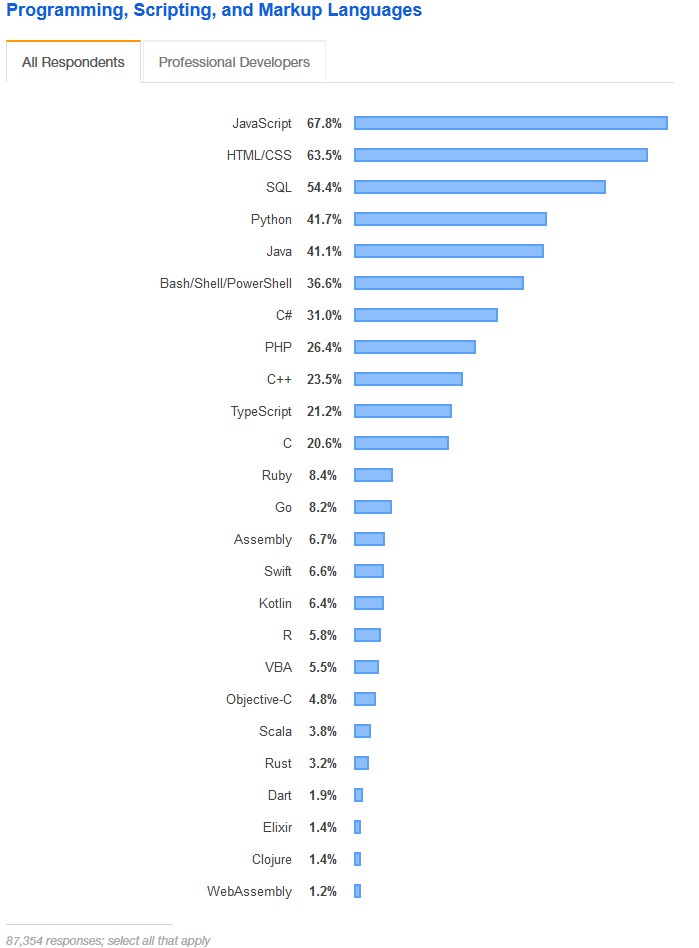
\includegraphics[width=0.95\textwidth]{images/chapter1/stackoverflow_language.png}
    \caption{Encuesta sobre lenguajes de programación usados en StackOverflow 2019.}
    \label{fig:Encuesta sobre lenguajes de programación en StackOverflow 2019}
\end{figure}

\subsection{Concepto Deep Learning}\label{subsec:concepto-deep-learning}
El \texit{Deep Learning} lleva consigo como principal actuador algoritmos que basan su estructura en redes neuronales artificiales, imitando el comportamiento que tienen las del ser humano y su sistema nervioso central.
La fuerza que ha proporcionado el surgimiento del Big Data ha conseguido que este tipo tecnologías se conviertan en la práctica diaría de muchos trabajadores.
Una de las claves de los algoritmos de \texit{Deep Learning} es en la capacidad de aprendizaje que reside en ellos.
Esto nos brinda la posibilidad de lidiar con problemas del mundo real,
en el que las combinaciones de posibilidades y reconocimiento de patrones se quedan fuera de nuestros cálculos.

Para poder materializar todos estos algoritmos de aprendizaje automático disponemos de servicios de grandes empresas como Google, Amazon, IBM, los cuales
implementan sus propias soluciones comerciales.
Pero también podemos optar por herramientas de código abierto como TensorFlow, una de las librerías más famosas de \texit{Deep Learning} desarrollada por los ingenieros de Google en primera instancia y posteriormente liberada bajo licencia Apache.
También disponemos de otras como PyTorch y Keras.
Todas las mencionadas anteriormente fueron originalmente desarrolladas para el lenguaje de programación Python, el cual ha visto aumentado su porcentaje de uso debido a esta corriente de
machine learning.

\subsection{Redes neuronales en el tratamiento de imágenes}\label{subsec:redes-neuronales-en-el-tratamiento-de-imágenes}
La unidad básica de procesamiento de las redes neuronales es el perceptrón (ver Figura~\ref{fig:Perceptrón}),
a partir del cual se desarrolla un algoritmo capaz de generar criterios de selección de subconjuntos de neuronas.
Este conjunto de neuronas pasará a formar parte de las distintas capas que componen por completo la red neuronal.
Cada neurona recibe una entrada, ya sea de una fuente externa o de otra neurona.

A partir de aquí cada neurona aplica una función de cálculo a partir de la cual se generan los pesos correspondientes de cada neurona. Estos pesos representan el nivel de interacción de las neuronas y deberán de ser ajustados de manera que se ciñan lo más posible a los datos que conocemos.
Los pesos de entrada de una capa tienen origen en una capa anterior y sus salidas forman parte de la entrada de una capa posterior, la propagación se produce hasta llegar a la última capa de la red, que será la capa de salida de la que obtengamos el resultado de nuestra clasificación.


\begin{figure}[H]
    \centering
    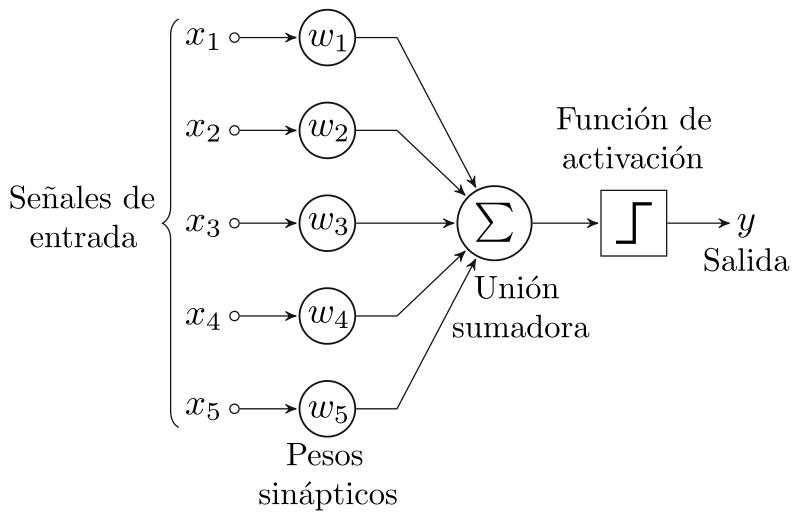
\includegraphics[width=0.6\textwidth]{images/chapter1/perceptron.png}
    \caption{Ejemplo de perceptrón.}
    \label{fig:Perceptrón}
\end{figure}

En este problema concreto nos centramos en clasificar imágenes multiespectrales con alta resolución espacial haciendo uso de las bandas espectrales RGB (Red, Green and Blue).
%cuyo objetivo consiste en la captura de datos de imágenes dentro de rangos de longitud de onda específicos a través del espectro electromagnético.
Nuestro conjunto de imágenes pertenece a una zona parcialmente destruida por un desastre natural en Haití ocurrido en el año 2010.
Estas imágenes fueron adquiridas por el satélite de observación terrestre de alta resolución GeoEye-1, lanzado en septiembre de 2008.
Por lo tanto, el fin de nuestro modelo de \texit{Deep Learning} es tener la capacidad de clasificar dichas imágenes dependiendo si la zona está dañada o, por el contrario, está en buenas condiciones.

\section{Plan de trabajo}\label{sec:plan-de-trabajo}


\section{Organización de esta memoria}\label{sec:organización-de-esta-memoria}

Teniendo presentes los anteriores objetivos concretos, se procede a describir la organización del resto de esta memoria, estructurada en una serie de capítulos cuyos contenidos se
describen a continuación:

\begin{itemize}
    \item \textbf{Entrenamiento del modelo mediante Google colab}: se define el proceso de entrenamiento y aumento de la velocidad del mismo usando la plataforma Google colab y su hardware asociado.
    \item \textbf{Tecnología OpenVINO}: se define el propósito del kit de herramientas de Intel OpenVINO así como la transformación de un modelo de TensorFlow para que sea compatible con dicha solución.
    \item \textbf{Arquitectura Cloud propuesta}: se presenta la arquitectura de Google Cloud diseñada para soportar toda la infraestructura de la aplicación y se explica la puesta en producción del servicio.
    \item \textbf{Resultados experimentales}: se preparan los distintos frameworks web que van a ser puestos a prueba haciendo uso del lenguaje de programación Python, mostrando el rendimiento obtenido en las fases de entrenamiento y de inferencias. Además, se presentará el cálculo aproximado de los costes del proyecto.
    \item \textbf{Conclusiones y trabajo futuro}: se presentan las conclusiones obtenidas mediante las pruebas de carga y también algunas posibles líneas de trabajo futuro que se pueden desempeñar en relación al presente trabajo.
\end{itemize}
    \mbox{}


\chapter{Entrenamiento del modelo mediante Google Colab}
\label{ch:chapter2}
Dentro del entrenamiento de modelos Deep Learning\cite{advanced_convolutional_network}, la velocidad es uno de los parámetros fundamentales.
Los modelos pueden requerir entradas de tamaño masivo en las que la capacidad de cómputo se torne clave para acelerar el proceso;
esto permite enfocarse plenamente en la mejora de rendimiento del modelo planteado.
El objetivo es evitar la posible espera que pueda producir volver a entrenar el mismo con distintos parámetros.
Con ello, se puede reajustar constantemente el modelo para encontrar el punto óptimo de manera ágil.

En este trabajo se va a entrenar un modelo de \texit{Deep Learning} haciendo uso del framework de código abierto de TensorFlow\footnote{\url{https://www.tensorflow.org/}}, que está programada en el lenguaje de programación Python.
Éste incluye una API de Deep Learning llamada Keras, que será la que utilicemos.
El tipo de operaciones que requiere nuestra aplicación en la parte del tratamiento de imágenes, así como los procedimientos que realizan las redes neuronales\cite{neural_network} para hacer sus cálculos son, en muchas ocasiones,
operaciones matriciales.

Nuestro objetivo será aprovechar al máximo el rendimiento que una GPU (Unidad de Procesamiento Gráfico) puede aportar en este tipo de operaciones, principalmente por su arquitectura de paralelización, idónea para este tipo de trabajo.
La ventaja que aporta frente a la CPU (Unidad de Procesamiento Central) es la capacidad de cómputo con un mayor número de núcleos o cores (ver Figura~\ref{fig:Arquitectura de paralelización de una GPU}), gracias a su conectividad por PCI express y el ancho de banda que esta proporciona.

Cabe mencionar que Google Colab, al ser una plataforma gratuita, no asegura la disponibilidad de sus componentes.
Esto conlleva que tanto el hardware requerido como su memoria disponible puede variar según la demanda del sistema.
En este trabajo se han matenido los mismos componentes hardware en Google Colab con la máxima memoria disponible.
\begin{figure}
    \centering
    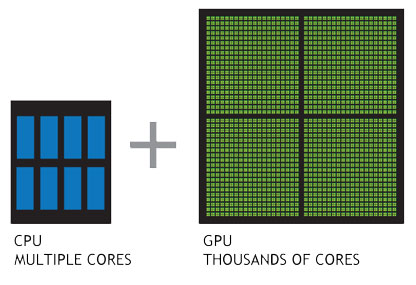
\includegraphics[width=0.5\textwidth]{images/chapter2/cpu-and-gpu.jpg}
    \caption{Diferencia de núcleos para procesar cargas de trabajo en paralelo de forma eficiente entre CPU y GPU.}
    \label{fig:Arquitectura de paralelización de una GPU}
\end{figure}


\section{Modelo propuesto}\label{sec:modelo-propuesto}
En esta parte del trabajo se pretende conseguir la máxima velocidad de entrenamiento posible manteniendo unos niveles de precisión elevados en la predicción.
Nuestro modelo tiene como cometido primordial poder clasificar distintas imágenes según el estado del terreno que aparece en la fotografía, siendo las opciones: terreno dañado y terreno en buenas condiciones. Para ello, disponemos de un dataset de 268 imágenes multiespectrales, adquirido por el satélite de observación terrestre de alta resolución GeoEye-1 durante el terremoto ocurrido en Haití en 2010. En este tipo de imágenes se capturan datos dentro de rangos de longitud de onda específicos a través del espectro electromagnético visible.

Como framework principal para realizar el entrenamiento nos ayudaremos de TensorFlow, que incluye la librería de \texit{Deep Learning} Keras, la cual simplifica mucho la implementación de este tipo de algoritmos de aprendizaje automático, debido a que sus objetos y funciones están programados de una manera intuitiva.
La distribución a efectuar sobre el conjunto de datos en entrenamiento y test es del 70\% y 30\% respectivamente.
Para la construcción de este modelo haremos uso de las siguientes capas, sobre las que TensorFlow nos da una API para tener control total sobre su configuración. Son descritas a continuación:

\begin{itemize}
    \item \textbf{Conv2D}: capa convolucional cuyo principal objetivo es extraer características de la imagen de entrada o partes de la misma.
    El térmido 2D se refiere al movimiento del filtro, el cuál es un parámetro de entrada de este tipo de capas.
    El filtro atraviesa la imagen en dos dimensiones.
    Tiene como parámetros de entrada una imagen en tres dimensiones y el número de filtros que vamos a aplicar sobre la imagen.
    Aplicaremos sobre esta capa una configuración de 64 filtros y un tamaño de kernel de 3$\times$3 ya que nuestras imágenes son de 128$\times$128 píxeles. Los filtros de mayor tamaño ayudarán al modelo a mejorar su aprendizaje.
    \item \textbf{Activación Relu (Recitified Linear Unit)}: en redes neuronales, una función de activación es la responsable de transformar la entrada.
    Sus principales funciones son detectar posibles correlaciones entre dos variables distintas dependiendo de sus valores y ayudar al modelo a tener en cuenta funciones no lineales, lo que significa, que la red neuronal es capaz de realizar microajustes para capturar relaciones entre entradas y salidas que no sigan una línea recta en el plano cartesiano.
    Como podemos observar en la Figura~\ref{fig:Función de activación Relu}, la función de activación Relu se comporta devolviendo un 0 para valores de entrada negativos y en caso contrario devolviendo el propio valor de entrada.
    Esta función de activación conserva los valores que contienen algún patrón en la imagen y los transfiere a la siguiente capa, mientras que los pesos negativos no son importantes y son establecidos con el valor 0.
    Otras funciones de activación como la función Sigmoide o Tanh modifican todos los valores de entrada, la función Relu mantendrá los valores de peso positivo para las capas posteriores.
    \item \textbf{MaxPooling2D}: es una capa que sigue un proceso de discretización basado en muestras, su objetivo es reducir la muestra de una representación de entrada mediante el acortamiento de sus dimensiones.
    En nuestro modelo aplicaremos una reducción a matrices de 2$\times$2.

    \begin{figure}
        \centering
        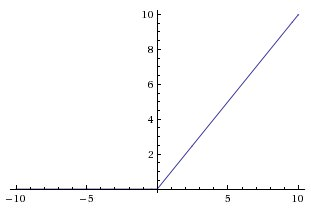
\includegraphics[width=0.5\textwidth]{images/chapter2/relu.jpg}
        \caption{Función de activación Relu.}
        \label{fig:Función de activación Relu}
    \end{figure}

    \item \textbf{Dropout}: es una capa cuyo cometido es ignorar ciertas neuronas de forma aleatoria para no incluirlas en el entrenamiento, por lo que las neuronas restantes serán las encargadas de representar las predicciones de la red.
    De esta manera también reducimos la complejidad de nuestra red y la posibilidad de sobreentrenamiento.
    \item \textbf{Flatten}: capa de aplanamiento usada para reducir a uno el número de dimensiones de nuestra matriz de entrada.
    \item \textbf{Dense}: una de las capas más utilizadas en la API de Keras, es la manera de efectuar multiplicaciones matriciales.
    \item \textbf{Optimizador Adam}: es un algoritmo de optimización diseñado especialmente para redes neuronales, este aprovecha el poder de los métodos de tasas de aprendizaje adaptativo para encontrar nivel de aprendizaje individuales para cada parámetro.
    Este optimizador posee un hyperparámetro llamado \textit{learning rate} que regula la rapidez con la que el modelo avanza hacia el valor optimo de sus pesos,
    un \textit{learning rate} bajo implicaría que los pesos evolucionan lentamente durante el entrenamiento, con lo cual puede tardarse mucho en llegar al valor optimo, mientras que con un learning rate alto avanzamos mas rapido pero podemos sobrepasar
    este punto óptimo. El valor de este hyperparámetro en este trabajo se mantiene a 0.0008.

\end{itemize}

Para un mejor entendimiento, en la Figura~\ref{fig:Topología de la red del modelo de redes neuronales.} podemos observar el conjunto de capas utilizado para crear la topología de la red de nuestro modelo. Además, algunas optimizaciones a nivel de hardware han sido realizadas para acelerar el proceso de forma general. Estas modificaciones son las siguientes:

\begin{figure}
    \centering
    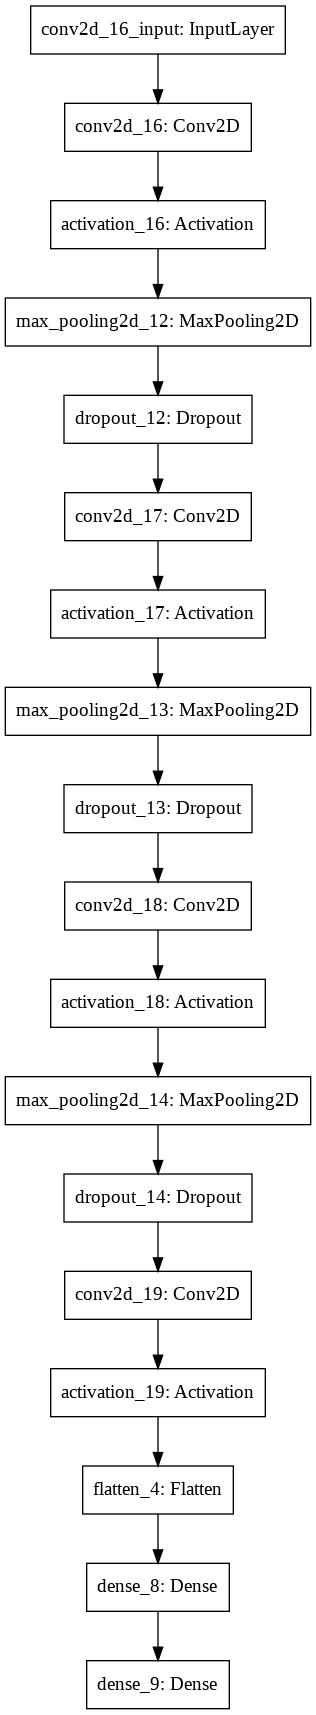
\includegraphics[width=0.2\textwidth]{images/chapter2/model.png}
    \caption{Topología de la red del modelo \texit{Deep Learning} usado para la clasificación de daños.}
    \label{fig:Topología de la red del modelo de redes neuronales.}
\end{figure}


\begin{itemize}
    \item \textbf{Uso de variables de 16 bits en vez de 32 bits}: una de las posibilidades que nos brinda el uso de una GPU es reducir a la mitad el uso en memoria de las variables del proceso.
    Usaremos esto siempre y cuando no afecte a la calidad de la predicción.
    \item \textbf{Uso del compilador XLA}: el compilador XLA\footnote{\url{https://www.tensorflow.org/xla}} (Accelerated Linear Algebra) optimiza el grafo de nuestro modelo de manera específica haciendo uso de la GPU.
    Normalmente cuando se ejecuta un Programa de TensorFlow cada operación tiene una implementación de kernel de GPU previamente compilada a la que el ejecutor envía datos.
    Con el compilador XLA conseguimos fusionar en una sola ejecución todas estas operaciones, consiguiendo así, reducir el el ancho de banda usado en memoria.
    \item \textbf{Valores altos del parámetro de entrenamiento Batch Size}: gracias a la capacidad de cómputo de nuestra GPU podemos permitirnos el uso de valores altos en este parámetro de entrenamiento.
\end{itemize}


\section{Entorno Google Colab}\label{sec:entorno-Google-colab}
La plataforma de Google Colab\footnote{\url{https://colab.research.Google.com/notebooks/intro.ipynb}} es un servicio gratuito de Google, mediante el cual podemos ejecutar e instalar librerías del lenguaje de programación Python\cite{python_object_oriented}.
Una de las grandes ventajas de trabajar con este entorno es que no necesitamos configuración ninguna, se ejecuta de forma íntegra en el navegador sin necesidad de instalar nada previamente y podemos compartir
nuestro trabajo con otras personas.
Estas características permiten a Google Colab convertirse en un entorno muy válido para personas que están dando sus primeros pasos en este área de la inteligencia artificial, pero haciendo uso
de unas herramientas profesionales.
En este trabajo haremos uso de la GPU Tesla K80\footnote{\url{https://www.nvidia.com/es-es/data-center/tesla-k80/}}.
Las características primarias de nuestra principal unidad de cómputo son las siguientes:
\begin{itemize}
    \item 4992 núcleos de NVIDIA CUDA con diseño de dos GPU\@.
    \item Hasta 2,91 teraflops de rendimiento en operaciones de precisión doble con NVIDIA GPU Boost.
    \item 24 GB de memoria GDDR5.
    \item 480 GB/s de ancho de banda de memoria agregado.
    \item Hasta 8,73 teraflops de rendimiento en operaciones de precisión simple con NVIDIA GPU Boost.
\end{itemize}

El uso de este tipo de herramientas en esta plataforma es extrapolable a otras nubes sin las restricciones en cuanto al número de unidades de procesamiento que necesitamos, la interoperabilidad de sus elementos con otros componentes externos, tales como servidores o respositorios de código, así como la configuración explícita de cada uno de los entornos de ejecución.
Una de las principales ventajas que tiene poder usar un entorno como Google Colab es que el servicio se ejecuta de manera íntegra online, de modo que toda la carga computacional reside en la herramienta de Google y no en nuestro computador.
Esto permite trabajar de manera fluida realizando otro tipo de cometidos en nuestra máquina, o simplemente ejecutar un proceso para el que no tenemos suficiente potencia disponible.

    \cleardoublepage
\mbox{}

\lstset{
language=Python,
basicstyle=\small\sffamily,
numbers=left,
numberstyle=\tiny,
frame=tb,
columns=fullflexible,
showstringspaces=false
}

\chapter{Tecnología OpenVINO}
\label{ch:chapter3}

OpenVINO es un conjunto de herramientas multi plataforma desarrolladas por Intel, que facilita la transición entre entre los entornos de entrenamiento y producción de nuestro modelo de aprendizaje profundo.
A pesar de estar desarrollada por una empresa comercial como Intel,peternece al conjunto de aplicaciones de código abierto, de modo que se puede visualizar su código fuente, repotar fallos e incluso realizar aportaciones.
Podemos visualizar el diseño y el código de la aplicación en su repositorio oficial de Github \footnote{https://github.com/openvinotoolkit/openvino}.
El cometido principal de esta aplicación es la optimización del tiempo de inferencia de un modelo de Deep Learning previamente entrenado.
Para ello, OpenVINO dispone de su propio formato de definición de modelos.
Estos archivos son los que procesa su propia red de inferencia multi plataforma, ya que se encuentra preparada para poder trabajar con los mismos de manera concurrente, aprovechando así toda la potencia de los procesadores o GPU actuales.
En la siguiente figura~\ref{fig:Arquitectura de optimización de modelos con OpenVINO} se puede observar el flujo de trabajo que se ha seguido en este trabajo, haciendo uso de la herramienta OpenVINO
En primer lugar, optimizaremos la topología de nuestro modelo a uno preparado para ser procesado por la red de inferencia de alto rendimiento de OpenVINO.
Finalmente, nuestra red de inferencia será la que realice el trabajo de clasificación en el entorno de producción de nuestra aplicació



\begin{figure}
    \centering
    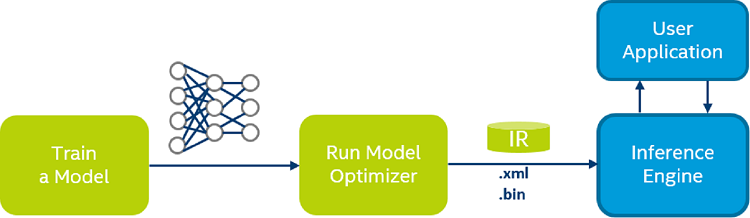
\includegraphics[width=0.8\textwidth]{images/chapter3/openvino_workflow.png}
    \caption{Arquitectura de optimización de modelos con OpenVINO}
    \label{fig:Arquitectura de optimización de modelos con OpenVINO}
\end{figure}


\section{Herramientas que lo componen}\label{sec:herramientas-que-lo-componen}
Esta tecnología desarrollada por intel tiene por objetivo principal la optimización de modelos de redes neuronales convolucionales para potenciar su velocidad de inferencia, mediante las distintas herramientas que lo componen.
OpenVINO es capaz de soportar distintos hardwares (FPGA, Intel movidius, procesamiento por GPU\@) y también varios sistemas operativos (Mac Os, Linux o Windows).
Las características principales de esta aplicación se resumen en dos puntos :
\begin{itemize}
    \item \textbf{Optimizador de modelos de deep learning}: Aplicación de interfaz de línea de comando, la cual usa como base modelos de frameworks populares como Caffe, TensorFlow, MXNet, Kaldi y ONNX para convertirlos a un modelo optimizado de OpenVINO.
    \item \textbf{Interfaz de inferencia de modelos de deep learning}: API de alto rendimiento multi plataforma para realizar la inferencia de manera rápida.
\end{itemize}

\subsection{Optimizador de modelos de deep learning}\label{subsec:optimizador-de-modelos-de-deep-learning}
Para poder realizar la optimización de nuestro modelo de deep learning previamente entrenado, se necesita el binario que contiene la topología de la red del modelo. Una vez el optimizador de OpenVINO recibe como argumento nuestro modelo procede a realizar una conversión de cada capa interna de la red a una nueva capa.
Esta nueva capa, ya convertida al formato de OpenVINO, conserva los pesos de la red anterior.
Sin embargo, la definición de la misma está preparada para que la aplicación de inferencia de OpenVINO pueda leerla correctamente.
La herramienta de OpenVINO proporciona de manera genérica distintos scripts para realizar esta conversión.
Se incluyen distintos scripts para los diferentes frameworks de Deep Learning más actuales, codificados en python y a los que se puede modifcar su código fuente, aunque en principio no es necesario porque ya vienen preparados para funcionar.

\subsection{Interfaz de infernecia de modelos de deep learning}\label{subsec:interfaz-de-infernecia-de-modelos-de-deep-learning}
Con nuestro modelo y su topología convertida a un formato válido de OpenVINO, ya tenemos todo lo necesario para poder realizar clasificaciones con la interfaz de inferencia de OpenVINO.
La optimización de inferencia se produce en este punto, donde cada capa de nuestro modelo original es procesada por la aplicación de inferencia en un lenguaje de bajo nivel, optimizado para realizar operaciones vectoriales bajo total control del programador.
El lenguaje empleado para la codificación de la aplicación es C++ pese a que el programa pueda ser utilizado también en Python.
Esto se debe al uso de su API, que traduce las peticiones realizadas en Python al core de la interfaz, que es C++ puro.
Todas las capas usadas en este proyecto son compatibles de manera directa con las predefinidas por la interfaz de inferencia.
Entre otras cosas, OpenVINO nos da la posibilidad de añadir capas personalizadas, con el inconveniente de que deben ser programadas por el usuario de manera explícita en C++ para hacerlas compatibles con el resto de la aplicación. Y, por supuesto, mantener estas nuevas capas a lo largo de las distintas actualizaciones y posibles cambios que pueda sufrir la aplicación.


\section{Conversión del modelo a la plataforma OpenVINO}\label{sec:conversión-del-modelo-a-la-plataforma-OpenVINO}
Para realizar la conversión del modelo, en primer lugar es necesaria la exportación del original de Tensorflow a un formato compatible con la red de optimización de modelos de OpenVINO.
La serialización por defecto de un modelo de Tensorflow puede incluir de manera independiente :

\begin{itemize}
    \item Un punto de control TensorFlow que contiene los pesos del modelo.
    \item Un prototipo 'SavedModel' que contiene el grafico subyacente de Tensorflow.
    Separa los graficos que se guardan para prediccion (servicio), capacitacion y evaluacion.
    Si el modelo no se compilo antes, solo el grafico de inferencia se exporta.
    \item La configuracion de arquitectura del modelo, si esta disponible
\end{itemize}

Los métodos exactos para la serializaciñon del modelo varían según la versión de Tensorflow, en cualquier caso la metodologíoa de conversión exacta utilizada
para este proyecto se puede encontrar en el repositorio de código fuente de este trabajo en Github : https://github.com/A-Ortiz-L/multispectral-imaging-cnn-final-degree-work
Este modelo de OpenVINO va a servir tanto de punto de partida para la optimización del mismo como para su uso directo en el servicio personalizado de Tensorflow para desplegar
modelos en producción.
Una vez exportado el modelo de deep learning al formato estándar de Tensorflow tendremos a nuestra disposición los ficheros necesarios para realizar la trasnformación de estos al formato de OpenVINO.
Para realizar esta operación se hace uso de la herramienta de Optimización de modelos, en concreto, con el script específico de Tensorflow, cuyo nombre
es \texttt{mo\_tf.py}

Este código fuente es ejecutado en la línea de comandos del sistema operativo correspondiente con los siguientes parámetros de entrada en la línea de comandos.


\begin{lstlisting}[caption=Comando de terminal para convertir un modelo Tensorflow a uno de OpenVINO.,
  label=a_label,
  float=t]
    mo_tf.py --input_model model.pb --input_model_is_text -b 1
\end{lstlisting}

En este comando epecifica con el flag \texttt{--input\_model\_is\_text} que nuestro fichero no está codificado en código binario, por lo que es texto plano.
Esta opción es totalmente configurable y depende del proceso de exportación.
Se ha encontrado útil la opción de exportaciòn a texto plano ya que de esta manera
se puede observar la arquitectura de la red y los pesos pertenecientes a cada capa.
Configuramos también el flag -b, esta opción determina el tamaño del batch que queremos especificar para la conversión, seleccionamos 1 porque en las entradas de nuestra red neuronal pueden propagarse valores
negativos, los cuales no son válidos para su procesamiento en OpenVINO.

\section{Inferencias.Tensorflow vs OpenVINO}\label{sec:inferencias.-Tensorflow-vs-OpenVINO}
Como se ha mencionado anteriormente Tensorflow posee su propio sistema de inferencia preparado para su uso productivo en un entorno real.
Esta sistema se llama Tensorflow serving, el cual incorpora un servidor codificado mediante el patrón diseño api rest, de modo que las peticiones
de inferencia se realizan al servidor por medio del protocolo de transmisión de datos http.
La aplicación de Tensorflow está diseñada para el escalado tanto en el número de modelos para los que puede recibir inferencias y sus versiones como para la escalabilidad en capacidad de cálculo.
El escalado de cáculo está preparado para funcionar en una arquitectura cluster, en este caso un cluster de contenedores como es kubernetes, por lo que el servidor puede ser
encapsulado en su totalidad en un contenedor de docker.
En este trabajo se ha trabajado con una versión encapsulada de docker, pero no con la extensibilidad del escalado con kubernetes.
La unidad de cálculo principal del sistema de inferncia también es configurable, perimitiendo así el uso tanto de cpu como de gpu.
Si se usa la opción de contenedores docker configurando una gpu es necesario configurar de manera esplícita este entorno.
En la siguiente figura podemos observar el diseño de la arquitectura de la aplicación~\ref{fig:Arquitectura de Tensorflow serving}
Una de las ventajas frente a usar el sistemá de inferencias clásico de Tensorflow es que la aplicación está preparada y optimizada para recibir tanto peticiones en streaming como en batch.
Adicionalmente reducimos el tamaño de las librerías a instalar al mínimo necesario para realizar las inferencias y configurar el servidor, por lo que la solución es más ligera y portable, evitando así
instalar todo el sistema de construcción de algoritmos y demás artefactos que incorpora la librerías de Tensorflow para construir redes neuronales.
La inicialización del servidor y los métodos necesarios para realizar la petición de inferencia se codifican de la siguiente manera :

\begin{lstlisting}[caption=Clase de Tensorflow de la aplicación del trabajo.,
  label=a_label,
  language=python]



class TensorflowNetwork:
    def __init__(self):
        self.model_uri = 'http://localhost:8501/v1/models/model:predict'
        self.init_tensorflow_serve()

    @staticmethod
    def shape_image(file_route):
        img_array = cv2.imread(file_route, cv2.IMREAD_GRAYSCALE)
        new_array = cv2.resize(img_array, (128, 128))
        img = new_array.reshape(-1, 128, 128, 1) / 255.0
        img = np.float32(img).tolist()
        return img

    def process_image(self, file_route) -> Tuple[bool, float]:
        start = time.time()
        image = self.shape_image(file_route)
        predict = self.network_request(image)
        return predict, (time.time() - start)

    def network_request(self, image) -> bool:
        headers = {"content-type": "application/json"}
        data = json.dumps({"signature_name": "serving_default", "instances": image})
        res = requests.post(self.model_uri, data=data,
                            headers=headers)
        predictions = json.loads(res.text)['predictions']
        predict = True if predictions[0][0] >= 0.5 else False
        return predict

    @staticmethod
    def init_tensorflow_serve():
        os.system('tensorflow_model_server '
                  '--rest_api_port=8501 --model_name=model '
                  '--model_base_path=/app/model &')
\end{lstlisting}
En la inicialización de la clase arrancamos el servidor rest, el cual funcionará de manera transparente para el usuario de nuestra aplicación, ya que el mismo se ejecuta en la red
local de nuestro servidor principal


\begin{figure}[h]
    \centering
    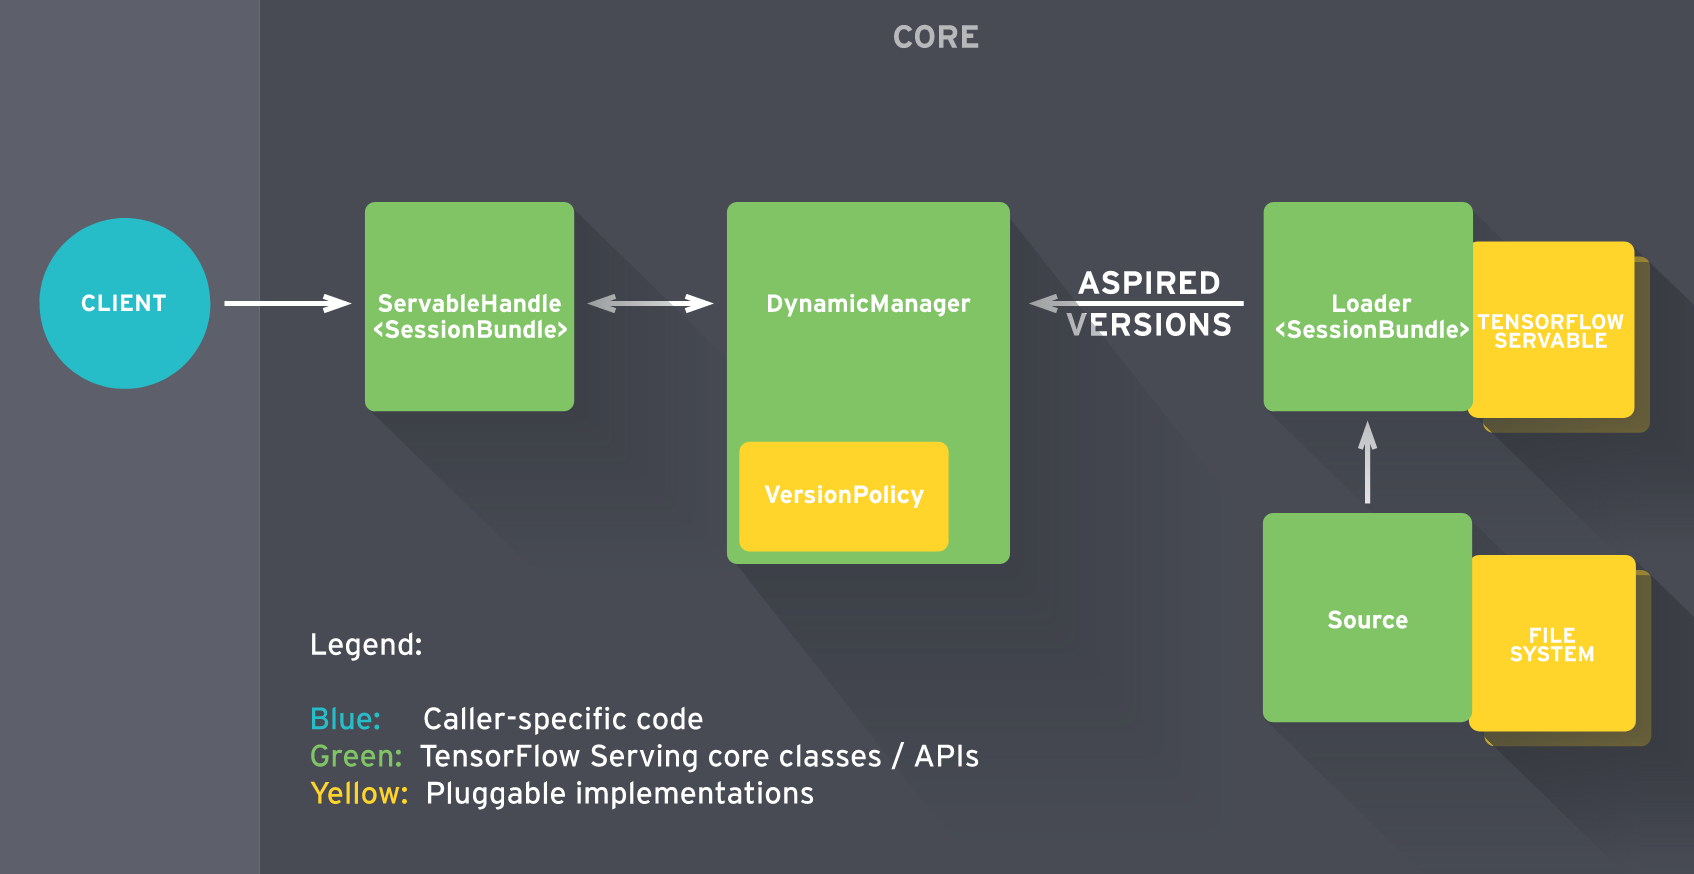
\includegraphics[width=0.8\textwidth]{images/chapter3/tf_serving_architecture.png}
    \caption{Arquitectura de Tensorflow serving}
    \label{fig:Arquitectura de Tensorflow serving}
\end{figure}

Por otro lado, OpenVINO también incorpora en su conjunto de herramientas un sistema de inferencia optimizado.
Al igual que el sistema de inferencia de Tensorflow, OpenVINO también puede configurar tanto cpu como gpu para realizar sus cálculos.
La aplicación de inferencia de OpenVINO usaada en este trabajo se codifica de manera íntegra haciendo uso del lenguaje de programación python,
por lo que el diseño software de este servicio y el procesamiento de las imágenes se codifica de la siguiente manera en el repositorio del trabajo.

\begin{lstlisting}[caption=Clase de OpenVINO de la aplicación del trabajo.,
  label=b_label,
  language=python]
    class OpenVinoNetwork:
    def __init__(self):
        self.plugin = IEPlugin(device='CPU')
        self.net = IENetwork(model=f'{pickle_dir}model.xml',
                             weights=f'{pickle_dir}model.bin')
        self.exec_net = self.plugin.load(network=self.net)

        self.input_blob = next(iter(self.net.inputs))
        self.out_blob = next(iter(self.net.outputs))
        self.net.batch_size = 1
        self.image_shape = 128

    def process_image(self, image_path) -> Tuple[bool, float]:
        start = time.time()
        image = self.shape_image(image_path)
        res = self.network_request(image)
        return res, time.time() - start

    def shape_image(self, file_route):
        image = cv2.imread(file_route, cv2.IMREAD_GRAYSCALE)
        image = cv2.resize(image, (self.image_shape, self.image_shape))
        image = image.reshape(self.image_shape, self.image_shape) / 255.0
        return image

    def network_request(self, image) -> bool:
        res = self.exec_net.infer(inputs={self.input_blob: image})
        res = res[self.out_blob]
        res = False if res < 0.5 else True
        return res
\end{lstlisting}

En la inicialización de la clase se lee el fichero ya optimizado del modelo de deep learning, también se inicia la clase
perteneciente a la api de inferencia de OpenVINO que se encarga de realizar las inferencia.
Se configuran métodos específicos para transformar la imagen a las dimensiones correspondientes y para hacer la petición a la red de inferencia.
La potencia de este modelo reside en la optimización que realiza la red en un lenguaje de bajo nivel, centrándose así en reducir los tiempos de inferencia.

En general, la aplicación de Tensorflow es más compleja a nivel de software, permitiendo su escalado en entornos de producción de manera muy simple.
Ambas soluciones implementan tecnologías de contenedores mantenidas de manera oficial por los fabricantes, por lo que el uso de Docker es la mejor opción para transportar
nuestras redes de inferencia a cuualquier sistema o dispositivo hardware.
En este punto, OpenVINO implementa de manera concreta soluciones para FPGA e intel movidius, por lo que las opciones de portabilidd son más amplias en esta tecnología.



    \cleardoublepage
\mbox{}

\chapter{Implementación}
\label{ch:chapter4}

\section{Descripción del entorno y sus diferentes componentes}
ok
\section{Codificación de los servidores web}
ok
\subsection{Framework FastApi}
ok
\subsection{Framework Flask}
oki
\section{Encapsulación de entorno con Docker}
(Explicación de las distintas imágenes de Docker de la aplicación y cómo se han construido)

    %\cleardoublepage
%\thispagestyle{empty}
\mbox{}

\chapter{Resultados experimentales}
\label{ch:chapte5}

\section{Dataset usado}
En cuanto a los tiempos de inferencia, la diferencia es notable entre ambos sistemas.
Los resultados se presentan haciendo uso de una mustra de 16.000 ejecuciones de inferencia en el entorno de producción de la aplicación, tanto para los entornos con Openvino, como para Tensorflow.
La unidad de cálculo principal es el procesador, siendo su modelo un Intel Xeon (Cascada Lake) con una frecuencia de 2.8 GHz de base y un turbo hasta 3.4 GHz.
Se han probado distintas configuraciones de este procesador, tanto en su versión de 2 núcleos físicos, 4 virtuales como en la de 4 núcleos físicos, 8 virtuales.
La memoria ram utilizada varía de 4 GB en su primera versión junto con el procesador de 2 núcleos físicos a 8 GB en la versión de 4 núcleos físicos.
ok
\section{Rendimiento en fase de entrenamiento}
ok
\section{Ren dimiento en fase de inferencias}
ok
\section{Costes del proyecto}
    \cleardoublepage
%\newpage
%\thispagestyle{empty}
\mbox{}

\chapter{Conclusiones y trabajo futuro}
\label{ch:chapte6}

\section{Conclusiones}\label{sec:conclusiones}
Los efectos de la globalizacion de internet son cada día más perceptibles en nuestras vidas.
El aumento de la población que interactúa por medio de apicaciones tiene como consecuencia la generación de una cantidad infinita de datos, que contienen toda la información de los usuarios que las emplean. Desde páginas web, aplicaciones móviles hasta sistemas que interactúan de manera automática, sin necesidad de que los usuarios tengan que usarlos o configurarlos. Hasta hace unos pocos años, estos ámbitos apenas escapaban de la esfera académica e investigadora, mientras que en los tiempos que corren se han convertido en una necesidad real de un mundo cada vez más interconectado a escala global.
A medida que crecen los datos en la red, aumenta la necesidad de su análisis y explotación.
Por ello, plataformas como Google Cloud, Amazon Web Services y similares llevan a cabo este proceso, bridando toda la potencia autogestionada de cómputo a los usuarios.
Diariamente nacen nuevas tecnologías de análisis específicas para estos datos.
Este es el caso de Tensorflow u OpenVINO, propiedad de empresas comerciales como Google o Intel.
La primera de ellas fue convertida a formato de código abierto, mientras que la segunda se situó como gratuita desde su lanzamiento;
ello da debida cuenta de la creciente comunidad que hace uso de estas herramientas.
Este tipo de recursos gratuitos, como Google Colab, otorgan a la comunidad de soluciones que solían ser de pago y accesible solo para cierto público dentro del sector tecnológico.
Y, al mismo tiempo, es esa misma comunidad la que reporta errores, propone actualizaciones o codifica directamente nuevas soluciones a incorporar.
Es la competitividad entre todas estas herramientas lo que impulsa una mejora constante en todas ellas.
Tensorflow nació como un framework enfocado en la generación de modelos de Deep Learning, pero no con el objetivo de principal de la puesta en producción de los modelos, como si hace OpenVINO. La simbiosis entre ambos crea una combinación completa que cubre las necesidades tanto de creación, como del uso de los modelos de aprendizaje profundo.
\section{Trabajo futuro}\label{sec:trabajo-futuro}
La plataforma se ha configurado de manera que su capacidad de procesamiento de peticiones sea escalable, esto es, porque el uso de la tecnología de contenedores dockerestá preparada para su integración en la solución de cluster Kubernetes\footnote{https://kubernetes.io/es/docs/concepts/overview/what-is-kubernetes/}.
La visualización de resultados en este trabajo ha sido realizada mediante los trabajos SQL en una base de datos, pero sería ideal poder contemplar los datos de una manera más intuitiva.
Docker nos permite portar fácilmente esta solución de contenedores a otros sistemas con distinto hardware, y, en consecuencia, puede funcionar de manera local sin tener una plataforma web o cloud que la soporte.
La clasificación podría producirse dentro del propio elemento que genera las imágenes, lo que eliminaría el tiempo de latencia de otros elementos adicionales.
En nuestro problema un vehículo aéreo podría portar el propio hardware de clasificación y sobrevolar el terreno dañado para clasificar las imágenes que va recogiendo.
Este sistema sería similar a opciones que ya se pueden encontrar en el mercado, como las AWS DeepLens{https://aws.amazon.com/es/deeplens/} de Amazon.
Los datos de este trabajo son imágenes RGB de una parte del planeta, por lo que tienen latitud y longitud exactas.
La técnica de visionado Heatmap\footnote{https://en.wikipedia.org/wiki/Heat_map} es la idónea para ver en tiempo real las zonas del terreno más afectadas por el desastre natural y poder redirigir los equipos de emergencia de manera rápida.
La configuración de los servidores ingesta las llamadas de manera interna, por lo que no está abierta a peticiones públicas de manera directa.
Si se decidiera abrir al público la clasificación de imágenes, habría que configurar en los servidores todos los certificados necesarios para funcionar con el protocolo seguro HTTPS. Además, ciertas medidas de seguridad contra factores como la denegación de servicio o intento de conexión no deseados a los servidores por los puertos abiertos de la aplicación, en nuestro caso 8080 y 22, que usamos para conectarnos por SSH.\footnote{https://es.wikipedia.org/wiki/Secure_Shell}.
    \bibliographystyle{unsrt}
    \bibliography{references}
    \addcontentsline{toc}{chapter}{Bibliografía}
    \cleardoublepage
    \appendix
    \cleardoublepage
    %\cleardoublepage
\newpage

\chapter{Introduction}
\label{Appendix:Introduccion}

\section{Motivation}

A hyperspectral image is a high spectral resolution image obtained through sensors capable of obtaining hundreds or even thousands of images on the same terrestrial area but corresponding to different wavelength channels. The set of spectral bands is not strictly limited to the visible spectrum but also covers the infrared and the ultraviolet.

At present, the use of hyperspectral images is increasing considerably due to the launching of new satellites and the interest in remote observation of the Earth, which has utility in areas as diverse as defense, precision agriculture, geology (detection of mineral deposits) , valuation of environmental impacts or even artificial vision.

During the last years there have been many advances with regard to sensor technology, which has revolutionized the collection, handling and analysis of the data collected. This evolution has managed to go from having a few tens of bands to having hundreds and the tendency is for the number to continue increasing. Institutions such as National Aeronautics and Space Administration (NASA) or the European Space Agency (ESA) are continuously obtaining a large amount of data that needs to be processed. As a result, new challenges have arisen in the processing of data.

If we add to the increase in the amount of information collected, many current and future remote observation applications require real-time processing capabilities (in the same time or less than the satellite takes to capture the data) or close to this real-time, it is essential to use parallel architectures for the efficient \cite{HPC_aplaza} and fast processing of this type of images.

The main problem in the processing of hyperspectral images lies in the spectral mixture, that is to say, the existence of mixed pixels in which several different materials coexist at the subpixel level. This type of pixels are the most common in hyperspectral images and for their analysis it is necessary to use complex algorithms with a high computational cost, which makes the execution of the demixing algorithms slow and requires acceleration or parallelization.

To address this type of tasks, parallel computing has been widely used through multi-core processors, GPUs (Graphics Processing Units) or dedicated hardware such as FPGAs (Field-Programmable Gate Arrays). Of all the alternatives, the latter present an efficient option in terms of performance, offering reduced times, in addition to a lesser use of resources, being the few alternatives that can be adapted in a sensor to perform on-board processing in space missions such as Mars Pathfinder or Mars Surveyor \cite{biblio:TFG_Esquembri}.

On the one hand, VHDL or Verilog are the native ways to program this type of devices, at a low level and more optimal. On the other hand, there is an alternative in OpenCL that allows a high level programming, faster and allowing its execution in a variety of architectures but less optimal at the level of hardware resources than in FPGAs devices.

\section{Objectives}

The general objective of this work is the parallel implementation on FPGA of the Automatic Target Detection and Classification Algorithm \cite{ATDCA, 298007} making use of the Gram Schmidt Orthogonalization and the programming languages VHDL and OpenCL. This will allow a very interesting comparison between a native language for said platform (VHDL) and another paradigm of parallel programming at a high level (OpenCL) that can be ported to other platforms such as multi-core processors, GPUs or other accelerators.

The achievement of the general objective is carried out in the present memory by addressing a series of specific objectives, which are listed below:

\begin{itemize}
    \item Design of individual modules in VHDL that serve to perform all the operations that are needed for the implementation of the ATDCA-GS algorithm.
    \item Elaboration of a state machine and implementation of the algorithm using the individual modules.
    \item Analysis and optimization of a previous parallel implementation in OpenCL of the algorithm.
    \item Obtaining results and performance comparisons between both programming languages.
\end{itemize}

\section{Organization of this memory}

Bearing in mind the previous specific objectives, we proceed to describe the organization of the rest of this report, structured in a series of chapters whose contents are described below:

\begin{itemize}
    \item \textbf{Hyperspectral analysis}: the hyperspectral image concept and the linear mixing model are defined; some hyperspectral sensors (AVIRIS and EO-1 Hyperion) and some spectral libraries (USGS and ASTER) are mentioned; and finally, the need for parallelization and platforms that can be used to address the problem of performance improvement is presented.
    \item \textbf{FPGAs technologies}: FPGA technologies are defined in a short way.
    \item \textbf{Implementation}: the algorithm ATDCA-GS in series is defined and the parallelization and optimization that has been carried out in both VHDL and OpenCL languages is explained.
    \item \textbf{Results}: the results obtained after the implementation and execution of the algorithm in FPGAs devices are presented.
    \item \textbf{Conclusions and future work}: the main conclusions of the aspects addressed in the work that have been reached and also some possible lines of future work that can be performed in relation to this work are presented.
\end{itemize}
    \cleardoublepage
\newpage
%\thispagestyle{empty}
\mbox{}

\chapter{Conclusions and future work}
\label{Appendix:Conclusion}

\section{Conclusions}

In this end-of-degree project, the design and implementation of the ATDCA-GS algorithm has been carried out, using Gram Schmidt orthogonalization in order to optimizing and improving the performance of complex operations such as the calculation of the inverse of a matrix. The programming languages VHDL and OpenCL have been used and the results of their execution in FPGA have been evaluated to subsequently make a performance comparison between both alternatives.

As part of the design, an adaptation of the algorithm to the usual flow of a specific hardware design has been carried out, minimizing as much as possible the amount of resources to be used and parallelizing the operations carried out during the execution of the algorithm.

To make a comparison in terms of the performance in time of the two implementations, it has been compared the acceleration of one with respect to the other making use of real and synthetic images. In addition, it has been verified that, except for the implementation in OpenCL for large images, the processing in both alternatives does not exceed the time limit (maximum) and therefore the real-time analysis can be performed, fulfilling one of the main objectives of this proyect.

The performance tests in terms of resources used in each implementation have revealed that the percentage of resources used increases linearly with the number of bands. It also revealed that for a large number of them (256), the resource with the highest use hardly reaches 86\% of use in VHDL and 48\% in OpenCL, so it is concluded that the performance is adequate.

\section{Lines of future work}

In the first place, it would be convenient to improve the implementation optimizations in OpenCL so that it allows a real-time analysis as well as the other alternatives. In addition, since the tendency of the size of the images is to continue growing more and more, the future work option that seems more evident is to be able to process other real images of an even larger size.

A possible future work path for this work would be to develop the algorithm by converting the floating-point arithmetic to whole arithmetic. In this way a better performance would be obtained since the calculations would be even simpler and, therefore, the number of necessary resources would decrease while increasing the clock frequency.

Another possible way of continuation could be the modification of the test platform to use the PCIe 3x8 bus. In this way penalties due to I / O would be reduced.

Finally, another way would be to choose whether the implementation kernels in OpenCL can follow a parallel programming model at task level, so that the task refers to the execution of a kernel with a work-group that contains a work-item and, thus, the compiler tries to accelerate the only work-item to get a better performance.
\end{document}
